\chapter{HASIL SEMENTARA}

Bab ini menyajikan hasil yang telah diperoleh sampai naskah ini disusun,
mengikuti rancangan dan prosedur yang ditetapkan pada Bab~III. Pembahasan
lengkap beserta seluruh tabel pengujian disajikan pada laporan akhir; bab ini
memuat hasil pokok yang sudah dapat disimpulkan.

\section{Cakupan Data dan Verifikasi Praanalisis}

Seluruh angka pada bab ini berasal dari satu matriks eksperimen yang dijalankan
pada 10 Agustus 2026 memakai model Qwen3-8B dengan $m=10$ langkah laten dan
rantai empat agen. Lengan \textit{benchmark} mencakup tiga tugas, masing-masing
dengan tujuh perlakuan, sehingga terdapat 21 sel utama, dan setiap sel
dievaluasi pada 100 soal.

Tiga verifikasi dijalankan sebelum analisis. Pertama, kesamaan soal antar-sel
diperiksa melalui sidik jari indeks soal; pada ketiga tugas, ketujuh sel
terbukti mengerjakan himpunan soal yang identik sehingga syarat uji berpasangan
terpenuhi. Kedua, konsistensi metadata run diperiksa dan tidak ditemukan
penyimpangan. Ketiga, kelengkapan berkas keluaran diperiksa terhadap daftar sel
yang direncanakan; satu sel acuan pada GSM8K kehilangan agregat pemakaian token
karena dijalankan sebelum mekanisme pengumpul transkrip dipasang, sedangkan
akurasi dan waktunya tetap tercatat.

Medium gabungan KV dan teks dijalankan pada subsampel kecil sebagai pemasok
transkrip lampiran, bukan sebagai sel eksperimen. Perbandingan medium pada bab
ini karena itu berlaku untuk medium teks, medium KV, dan konfigurasi agen
tunggal.

\section{Perbandingan Persamaan Langkah Laten}

\begin{table}[htbp]
\centering
\caption{Hasil lengan \textit{benchmark}: akurasi, biaya token, dan waktu untuk tujuh perlakuan pada tiga tugas ($n=100$ soal identik per tugas, Qwen3-8B, $m=10$ langkah laten). Kolom \textsc{Selisih} membandingkan rerata empat anggota keluarga relaksasi terhadap \texttt{raw} pada medium KV.}
\label{tab:hasil-bench}
\small
\begin{tabular}{llrrrrrrrr}
\hline
 & & \multicolumn{2}{c}{Acuan} & \multicolumn{5}{c}{Medium KV} & \\
\cline{3-4}\cline{5-9}
Tugas & Metrik & Tunggal & Teks & \texttt{raw} & \texttt{soft} & \texttt{gumbel} & \texttt{sample} & \texttt{moi} & Selisih \\
\hline
\multirow{3}{*}{GSM8K} & Akurasi & 0,92 & 0,90 & 0,83 & 0,88 & 0,91 & 0,86 & \textbf{0,92} & +0,062 \\
& Token & --- & 845 & 212 & 192 & 197 & 187 & 190 &  \\
& Waktu (dtk) & 15,7 & 49,2 & 19,7 & 14,5 & 28,1 & 16,5 & 15,9 &  \\
\hline
\multirow{3}{*}{ARC-C} & Akurasi & 0,91 & 0,93 & 0,89 & \textbf{0,94} & 0,91 & \textbf{0,94} & 0,91 & +0,035 \\
& Token & 271 & 1081 & 219 & 154 & 154 & 146 & 145 &  \\
& Waktu (dtk) & 20,3 & 76,0 & 20,6 & 14,0 & 15,9 & 13,3 & 15,3 &  \\
\hline
\multirow{3}{*}{HumanEval+} & Akurasi & 0,72 & 0,76 & 0,42 & 0,69 & 0,71 & \textbf{0,74} & 0,72 & +0,295 \\
& Token & 122 & 997 & 177 & 122 & 131 & 126 & 122 &  \\
& Waktu (dtk) & 10,9 & 69,3 & 17,8 & 11,4 & 14,9 & 12,4 & 14,1 &  \\
\hline
\end{tabular}
\end{table}


Tabel~\ref{tab:hasil-bench} menyajikan akurasi, biaya token keluaran per soal,
dan waktu per soal untuk ketujuh perlakuan pada ketiga tugas.
Gambar~\ref{gbr:hasil-utama} menampilkan ketiga metrik yang sama secara grafis.

\begin{figure}[htbp]
    \centering
    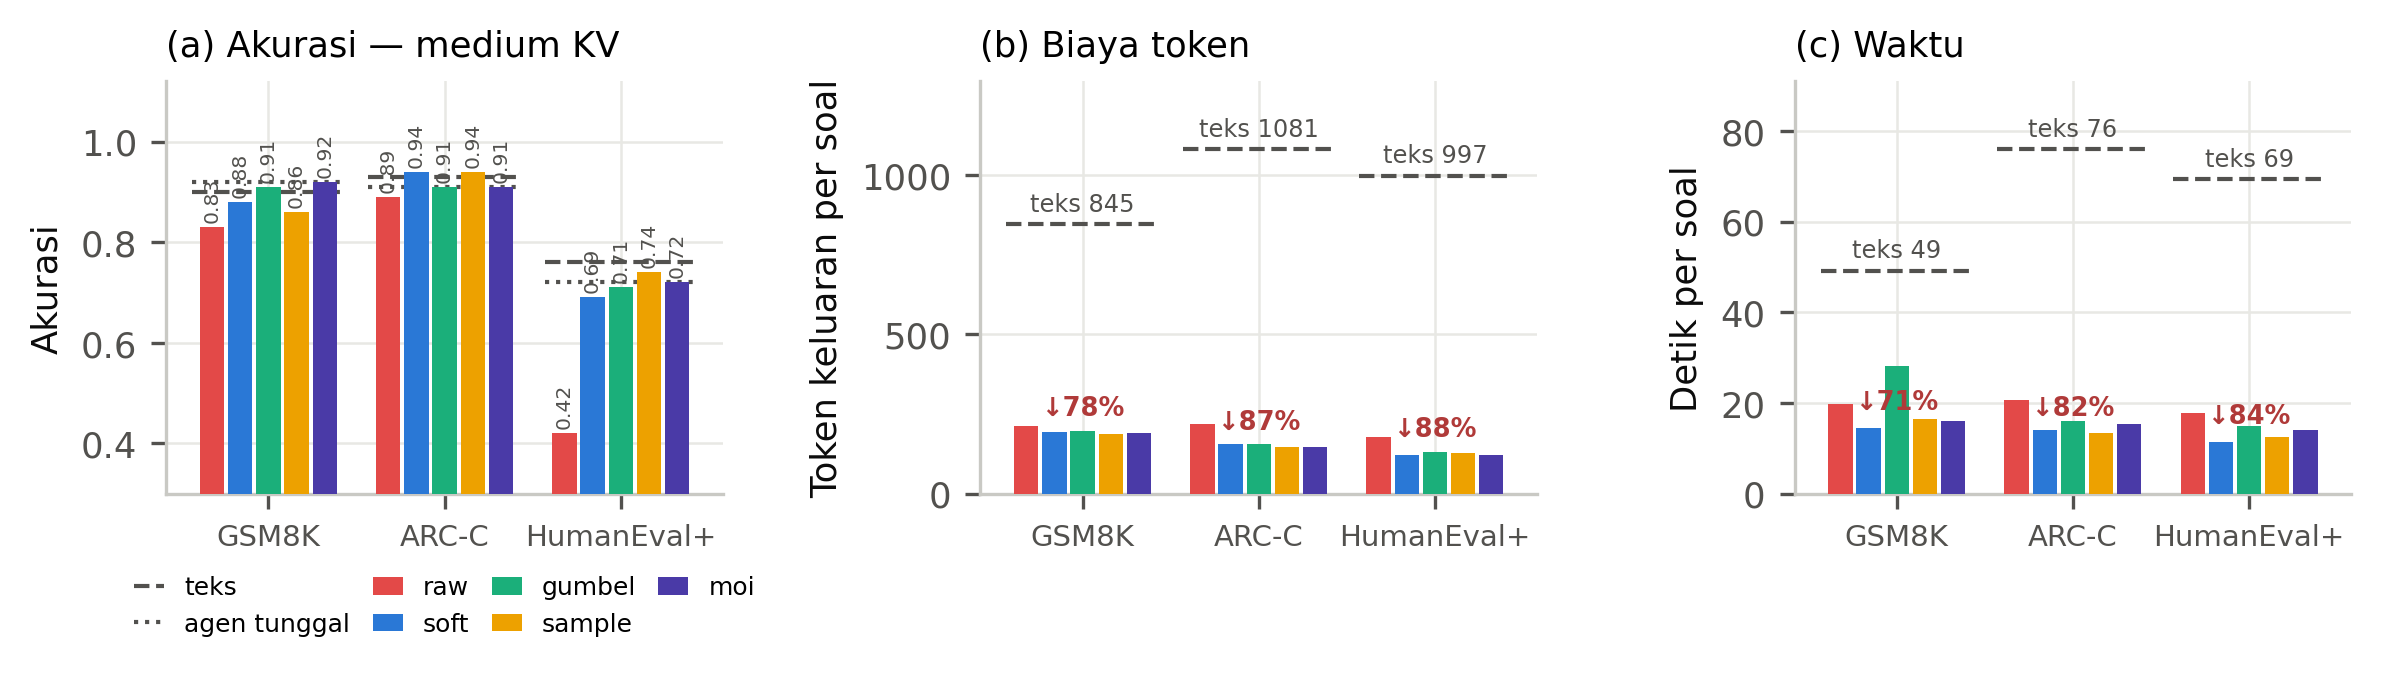
\includegraphics[width=\textwidth]{assets/images/hasil_utama.png}
    \caption{Akurasi, biaya token, dan waktu per soal pada medium KV untuk lima
    persamaan langkah laten. Garis putus-putus menandai medium teks dan garis
    titik-titik menandai agen tunggal.}
    \label{gbr:hasil-utama}
\end{figure}

Pola akurasinya berbeda tajam antar-tugas. Pada GSM8K dan ARC-C ketujuh
perlakuan berada dalam rentang sempit, yaitu 0,83--0,92 dan 0,89--0,94. Pada
HumanEval+ enam perlakuan berada pada 0,69--0,76, sementara persamaan langkah
laten resmi \code{raw} pada medium KV hanya mencapai 0,42.

Setiap pasangan perlakuan dalam satu tugas diuji dengan uji McNemar eksak,
sehingga seluruhnya terdapat 63 pengujian. Delapan pasangan signifikan pada
taraf nominal dan enam bertahan setelah koreksi Holm. Keenamnya berasal dari
HumanEval+ dan seluruhnya melibatkan \code{raw} pada medium KV; tidak ada satu
pun pasangan pada GSM8K maupun ARC-C yang bertahan, dan tidak ada satu pun
pasangan antar-anggota keluarga relaksasi yang bertahan pada tugas mana pun.

\begin{table}[htbp]
\centering
\caption{Seluruh pasangan yang tetap signifikan setelah koreksi Holm atas 63 uji McNemar eksak. Tak satu pun pasangan pada GSM8K dan ARC-C bertahan; seluruh pasangan yang bertahan berasal dari HumanEval+ dan melibatkan \texttt{raw} pada medium KV.}
\label{tab:uji-signifikan}
\small
\begin{tabular}{llrrrr}
\hline
Tugas & Pasangan & $\Delta$ & SK 95\% & $p$ & $p_{\text{Holm}}$ \\
\hline
HumanEval+ & \texttt{raw/kv} vs \texttt{sample/kv} & -0,320 & [-0,42; -0,22] & $1,9\times 10^{-8}$ & $1,2\times 10^{-6}$ \\
HumanEval+ & \texttt{moi/kv} vs \texttt{raw/kv} & +0,300 & [+0,20; +0,40] & $6,9\times 10^{-8}$ & $4,3\times 10^{-6}$ \\
HumanEval+ & \texttt{raw/baseline} vs \texttt{raw/kv} & +0,300 & [+0,20; +0,40] & $2,3\times 10^{-7}$ & $1,4\times 10^{-5}$ \\
HumanEval+ & \texttt{raw/kv} vs \texttt{raw/text} & -0,340 & [-0,45; -0,22] & $3,1\times 10^{-7}$ & $1,9\times 10^{-5}$ \\
HumanEval+ & \texttt{gumbel/kv} vs \texttt{raw/kv} & +0,290 & [+0,19; +0,40] & $1,1\times 10^{-6}$ & $6,4\times 10^{-5}$ \\
HumanEval+ & \texttt{raw/kv} vs \texttt{soft/kv} & -0,270 & [-0,37; -0,17] & $3,5\times 10^{-6}$ & $2,0\times 10^{-4}$ \\
\hline
\end{tabular}
\end{table}


Uji Cochran $Q$ atas kelima persamaan memberikan kesimpulan yang sejalan.
Hipotesis kesamaan kelima persamaan tidak dapat ditolak pada GSM8K
($Q = 7{,}40$; db $= 4$; $p = 0{,}116$) maupun ARC-C ($Q = 6{,}71$; db $= 4$;
$p = 0{,}152$), tetapi ditolak kuat pada HumanEval+ ($Q = 65{,}67$; db $= 4$;
$p < 0{,}0001$).

\section{Keterbedaan Hasil menurut Jenis Tugas}

\begin{figure}[htbp]
    \centering
    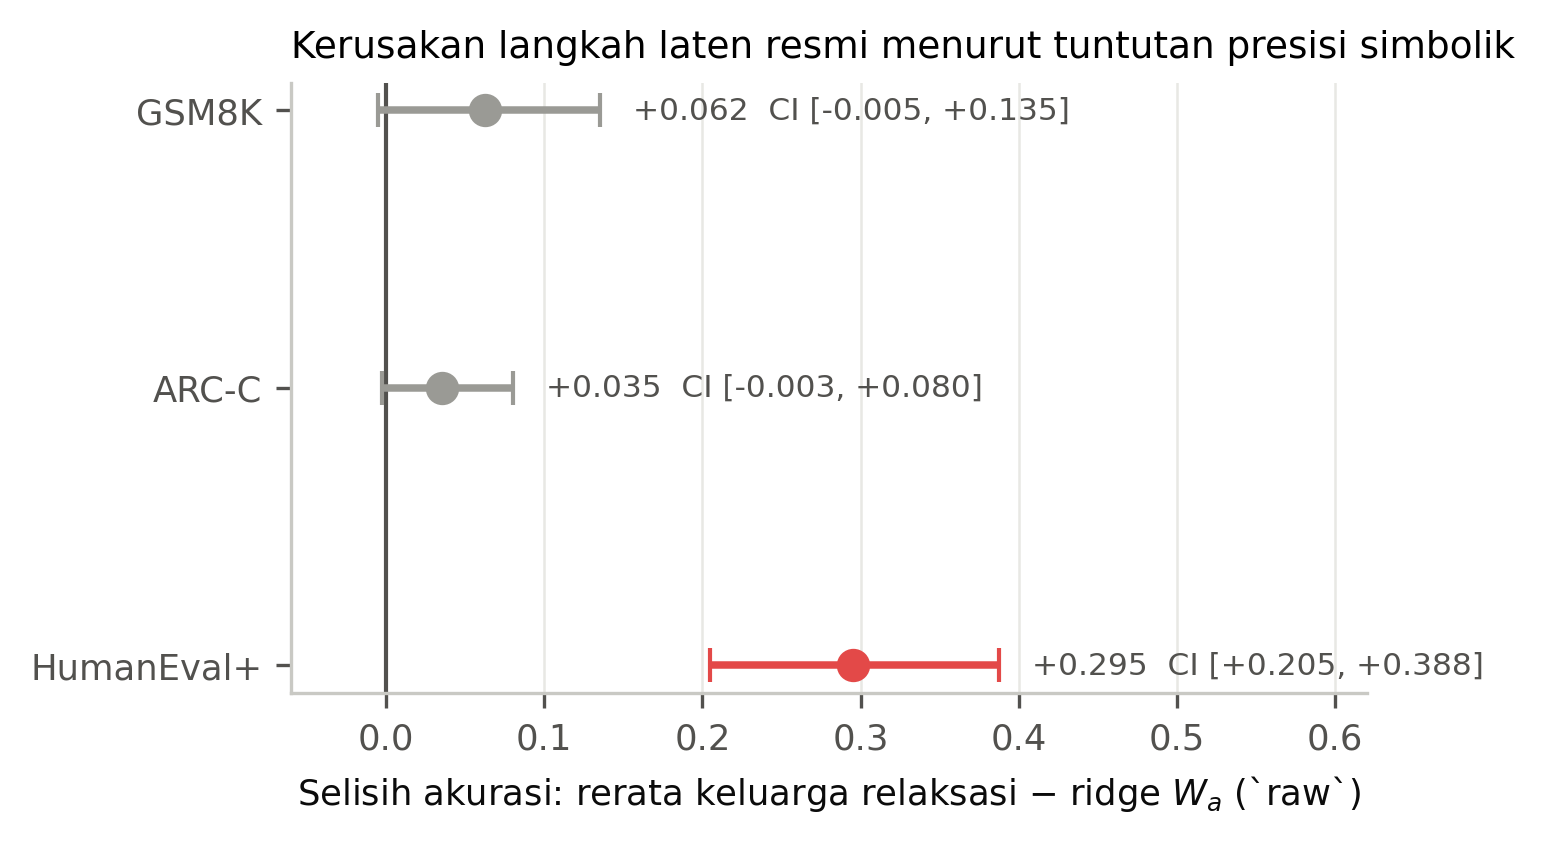
\includegraphics[width=0.85\textwidth]{assets/images/disosiasi.png}
    \caption{Selisih akurasi antara rerata keluarga relaksasi diskret dan ridge
    $W_a$ pada ketiga tugas, dengan selang kepercayaan \textit{bootstrap} 95\%.}
    \label{gbr:disosiasi}
\end{figure}

Selisih akurasi antara rerata keempat anggota keluarga relaksasi dan
\code{raw} adalah $+0{,}062$ pada GSM8K dan $+0{,}035$ pada ARC-C, keduanya
dengan selang kepercayaan yang memuat nol, sedangkan pada HumanEval+ selisihnya
$+0{,}295$ dengan selang kepercayaan $[+0{,}205; +0{,}388]$.

Perbandingan antar-tugas menegaskan keterbedaan tersebut. Kerusakan pada
HumanEval+ berbeda meyakinkan dari kerusakan pada GSM8K ($\Delta\Delta =
+0{,}232$; $p = 0{,}0002$) maupun ARC-C ($\Delta\Delta = +0{,}260$;
$p < 0{,}0001$), sementara GSM8K dan ARC-C tidak dapat dibedakan satu sama lain
($p = 0{,}542$).

Hasil ini mengonfirmasi sebagian hipotesis H2. Bagian yang terkonfirmasi adalah
keterbedaan itu sendiri, yaitu bahwa tugas dengan tuntutan presisi simbolik
tertinggi mengalami kerusakan jauh lebih besar. Bagian yang tidak terkonfirmasi
adalah urutan tiga tingkat yang diramalkan, karena GSM8K dan ARC-C tidak
berbeda satu sama lain; yang didukung data adalah pembedaan dua tingkat.

Satu pembacaan alternatif dapat ditutup di sini. Kerusakan pada HumanEval+ tidak
dapat dinisbahkan kepada medium KV, karena pada tugas yang sama empat perlakuan
lain yang juga memakai medium KV mencapai 0,69--0,74, yaitu setara dengan agen
tunggal (0,72) dan medium teks (0,76). Yang membedakan sel yang runtuh dari
keenam sel lainnya adalah persamaan langkah latennya, bukan mediumnya.

\section{Biaya Komputasi Medium Laten}

\begin{table}[htbp]
\centering
\caption{Efisiensi medium KV relatif terhadap medium teks, per persamaan langkah laten. Penghematan token dihitung atas token keluaran per soal; percepatan atas waktu dinding per soal. Kolom akurasi diulang dari Tabel~\ref{tab:hasil-bench} supaya biaya dan mutu terbaca pada satu baris.}
\label{tab:efisiensi}
\small
\begin{tabular}{llrrr}
\hline
Tugas & Langkah laten & Akurasi & Penghematan token & Percepatan \\
\hline
ARC-C & \texttt{raw} & 0,89 & 79,7\% & $\times3,7$ \\
ARC-C & \texttt{soft} & 0,94 & 85,7\% & $\times5,4$ \\
ARC-C & \texttt{gumbel} & 0,91 & 85,7\% & $\times4,8$ \\
ARC-C & \texttt{sample} & 0,94 & 86,5\% & $\times5,7$ \\
ARC-C & \texttt{moi} & 0,91 & 86,6\% & $\times5,0$ \\
\hline
GSM8K & \texttt{raw} & 0,83 & 75,0\% & $\times2,5$ \\
GSM8K & \texttt{soft} & 0,88 & 77,2\% & $\times3,4$ \\
GSM8K & \texttt{gumbel} & 0,91 & 76,7\% & $\times1,8$ \\
GSM8K & \texttt{sample} & 0,86 & 77,8\% & $\times3,0$ \\
GSM8K & \texttt{moi} & 0,92 & 77,5\% & $\times3,1$ \\
\hline
HumanEval+ & \texttt{raw} & 0,42 & 82,3\% & $\times3,9$ \\
HumanEval+ & \texttt{soft} & 0,69 & 87,8\% & $\times6,1$ \\
HumanEval+ & \texttt{gumbel} & 0,71 & 86,9\% & $\times4,7$ \\
HumanEval+ & \texttt{sample} & 0,74 & 87,4\% & $\times5,6$ \\
HumanEval+ & \texttt{moi} & 0,72 & 87,8\% & $\times4,9$ \\
\hline
\end{tabular}
\end{table}


Tabel~\ref{tab:efisiensi} menunjukkan penghematan token keluaran
75,0\%--87,8\% dan percepatan $\times 1{,}8$--$\times 6{,}1$ terhadap medium
teks. Rentang tersebut memuat rentang 70,8\%--83,7\% yang dilaporkan kerangka
LatentMAS \citep{latentmas}, sehingga klaim efisiensinya terreplikasi pada
implementasi dan perangkat keras yang berbeda.

Mekanisme penghematannya terbaca dari jumlah panggilan model: pada medium teks
setiap soal memicu empat panggilan berkeluaran teks, sedangkan pada medium KV
hanya satu, karena tiga agen perantara menyerahkan pekerjaan lewat
KV-\textit{cache} tanpa memverbalkan penalarannya.

Keunggulan biaya tersebut tidak disertai keunggulan akurasi. Terhadap medium
teks, akurasi sel KV terbaik lebih tinggi pada ARC-C dan GSM8K tetapi lebih
rendah pada HumanEval+, dan tak satu pun selisih tersebut signifikan. Rumusan
yang didukung data adalah kesetaraan akurasi pada biaya yang jauh lebih rendah.

\section{Bukti Mekanisme}

\begin{table}[htbp]
\centering
\caption{Geometri vektor langkah laten pada Qwen3-8B. Kolom terakhir adalah kosinus terhadap baris matriks embedding masukan yang paling dekat; nilai $1$ berarti vektor tepat berimpit dengan embedding sebuah token.}
\label{tab:geometri}
\small
\begin{tabular}{lccc}
\hline
Langkah laten & Bentuk & Anggota ($\star$) & $\max_i \cos(\Phi(h), W_{\text{in}}[i])$ \\
\hline
\texttt{raw} & $\rho\,hM/\lVert hM\rVert$ & tidak & 0,312 [0,16; 0,38] \\
\texttt{soft} & $w = p$ & ya & 0,927 [0,78; 1,00] \\
\texttt{gumbel} & $w = \mathrm{softmax}((\ell+g)/T)$ & ya & 0,985 [0,86; 1,00] \\
\texttt{sample} & $w = e_y$ & ya & 1,000 [1,00; 1,00] \\
\hline
\multicolumn{4}{l}{\footnotesize $\lVert M-I\rVert_F/\lVert I\rVert_F = 1,04$;\quad $\cos(h, hM)$ rerata $= 0,0112$;\quad $\cos(W_{\text{in}}[i], W_{\text{out}}[i])$ rerata $= 0,0041$.} \\
\end{tabular}
\end{table}


Pola di atas sejalan dengan sifat geometris kelima persamaan.
Tabel~\ref{tab:geometri} melaporkan kosinus antara vektor langkah laten dan
baris embedding masukan terdekat: anggota keluarga relaksasi berada pada
0,927--1,000, sedangkan \code{raw} hanya 0,312. Simpangan relatif matriks
realignment terhadap identitas mencapai 1,04 dan kosinus antara \textit{hidden
state} dan hasil pemetaannya hanya 0,0112, sehingga pemetaan tersebut memang
memindahkan vektor jauh dari titik asalnya tanpa mendaratkannya di dekat
embedding token mana pun.

Bukti pendukung berasal dari pengukuran kapasitas kanal yang dilakukan sebelum
lengan \textit{benchmark} dijalankan. Pada kanal laten murni yang membawa nama
fungsi sebagai muatan, persamaan \code{raw} memberikan \textit{recall} 0,000,
sedangkan keempat anggota keluarga relaksasi berada pada 0,34--0,38 dengan
$m=10$. Urutan kerusakan yang kemudian teramati pada lengan \textit{benchmark}
karena itu berstatus ramalan yang diuji, bukan penjelasan yang disusun setelah
melihat angka.

\section{Batas Berlaku Hasil Sementara}

Hasil pada bab ini diperoleh dari satu \textit{backbone} (Qwen3-8B), satu
\textit{seed} per sel, dan subsampel 100 soal per tugas, sehingga ragam
antar-\textit{seed} tidak terukur dan selang kepercayaan yang dilaporkan hanya
mencakup ragam antar-soal. Medium gabungan KV dan teks belum diuji pada ukuran
sampel yang memadai. Urutan tiga tingkat yang diramalkan pada rancangan tidak
terkonfirmasi; yang didukung data adalah pembedaan dua tingkat, yaitu tugas
pembangkitan kode terhadap kedua tugas lainnya. Analisis lengan faktor simbolik
dan pengujian fidelitas simbolik secara rinci disajikan pada laporan akhir.
